\section{Efficiency for electrons and muons}\label{sec:eff}

The efficiency ratio is derived directly from the data
but selection of an inclusive Z boson sample.
For this we select di-lepton events ($ee$, $\mu\mu$) 
with (20,10) GeV including the lepton trigger paths
listed in Sec.??.

We apply an cut in the invariant mass of $60 < m_{ll} < 120$~GeV
to obtain a pure Z boson sample. The differnt flavour subtraction 
described in Sec.~\ref{sec:ofossubtraction} relies on the 
knowledge of the electron to muon efficiency ratio, which
we derive from this sample as
\be
    r_{\mu e} = \sqrt{\frac{n_{\mu\mu}}{n_{ee}}} = 1.13 \pm 0.07
\ee

\begin{figure}[hbtp]

  \subfigure[]{\label{fig:cont_iOSee}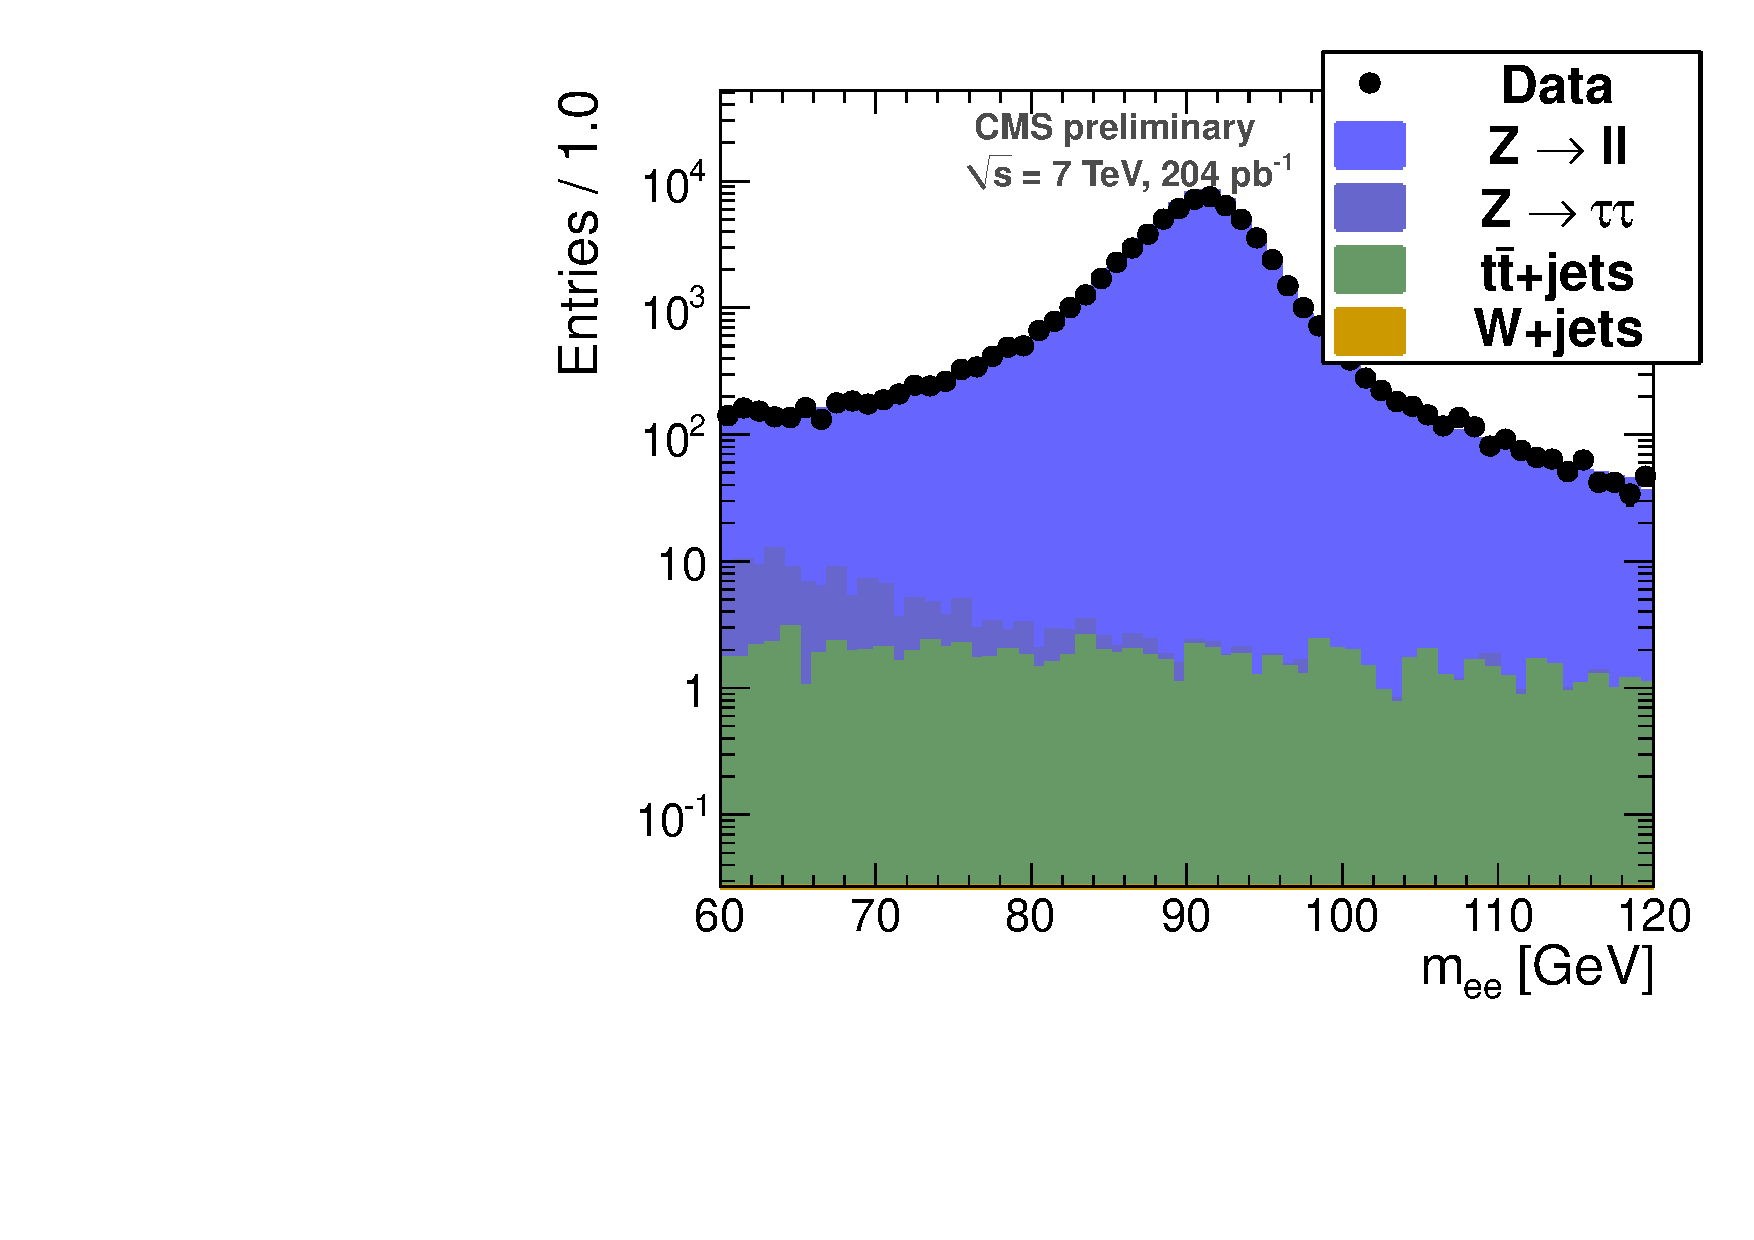
\includegraphics[width=0.49\textwidth]{Summer11_07_MC_pfLeptSusyCuts_Data_iOSee_EE.pdf}}\hfill
  \subfigure[]{\label{fig:cont_iOSmm}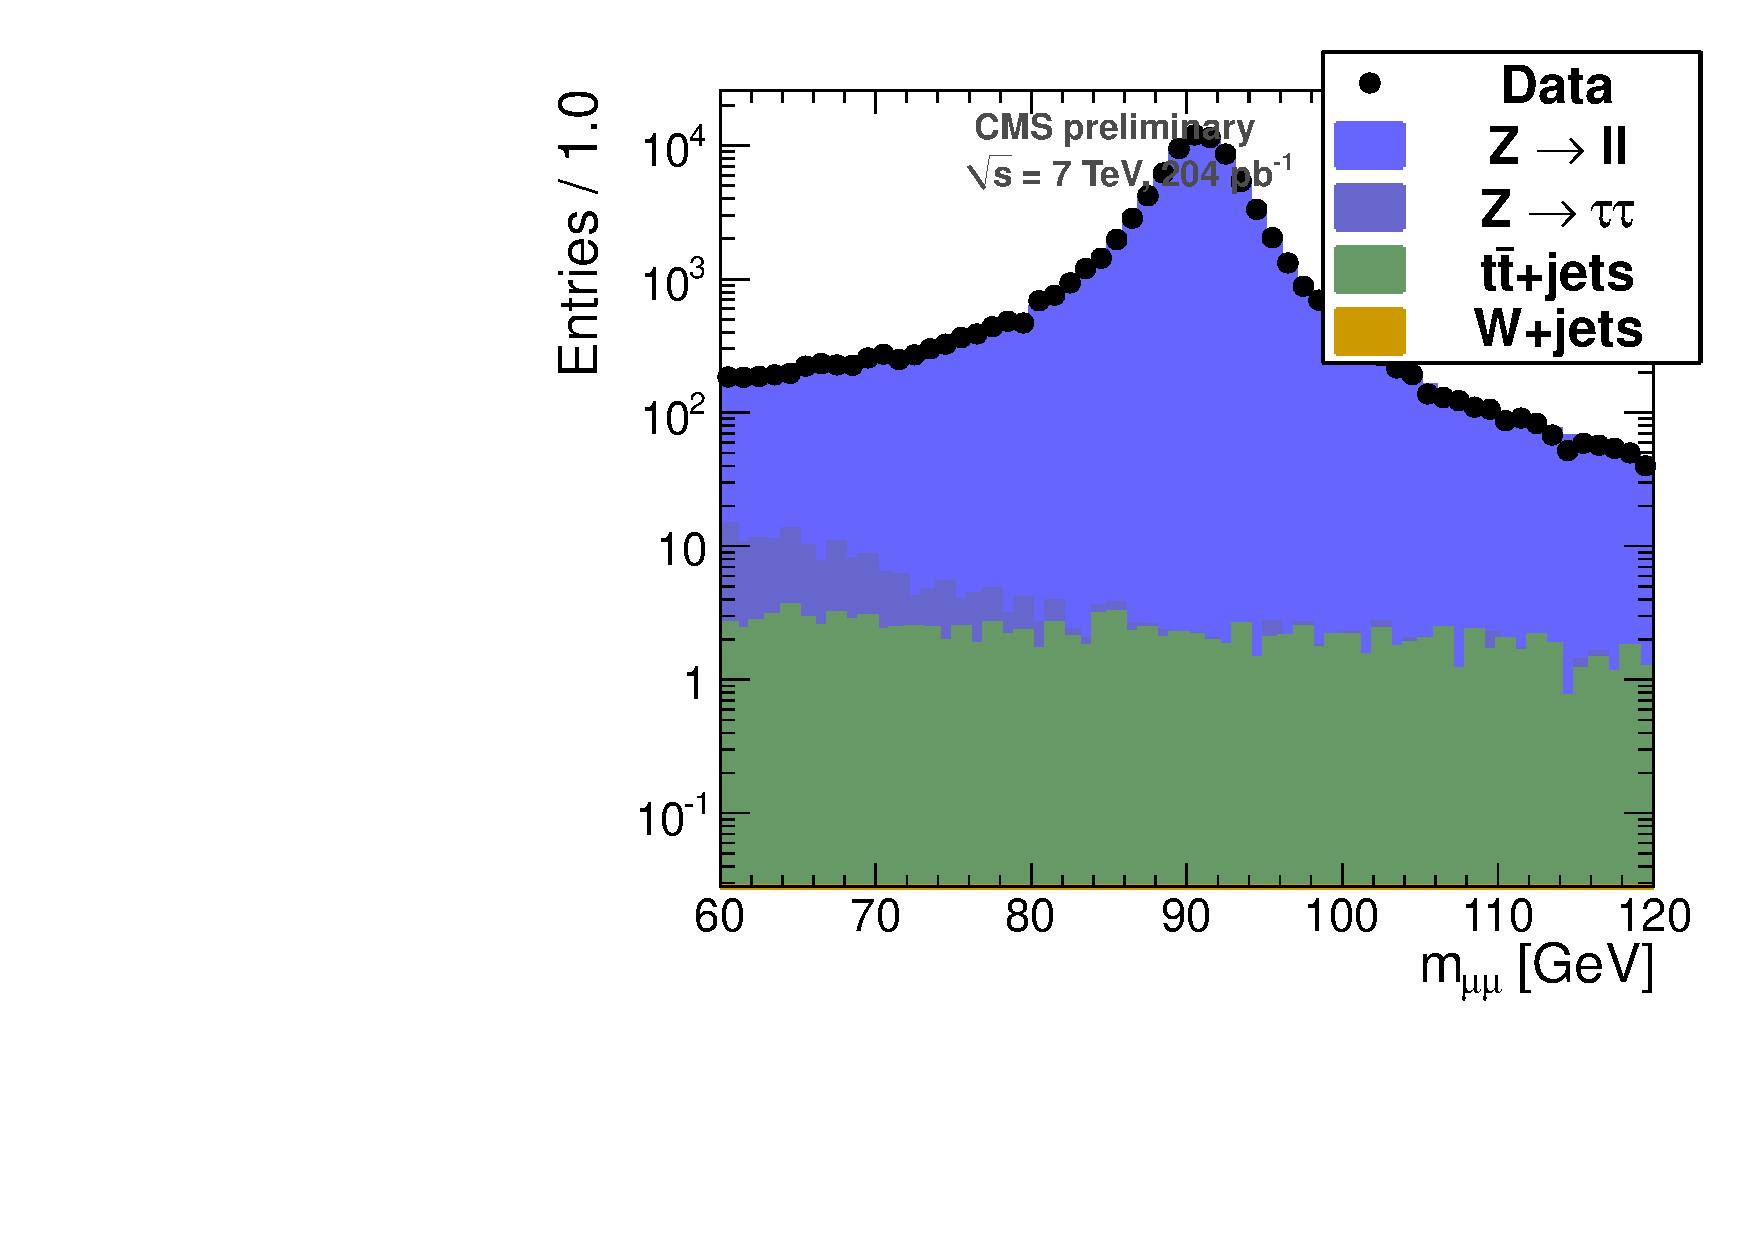
\includegraphics[width=0.49\textwidth]{Summer11_07_MC_pfLeptSusyCuts_Data_iOSmm_MuMu.pdf}}\hfill
  \caption{Invariant mass distributions for a (20,10) GeV di-lepton selection after leptonic 
      trigger requirement.\label{fig:Z_InvMass}}
\end{figure}


\begin{table}[htbp]
\begin{center}
\caption{\label{tab:tnp_eff}Muon to electron reconstruction efficiency ratio 
    obtained from a Z boson selection on data and $Z+\textrm{jets}$ Monte Carlo simulation.} 
\begin{tabular}{lcc}
\hline
            &  Data                                                 & Monte Carlo \\
\hline\hline
\hline
ratio $r_{\mu e}$       & $1.07 \pm 0.005 (\textrm{stat}) \pm 0.05 (\textrm{syst})$    & $1.052 \pm 0.003(\textrm{stat}) $ \\
\hline
\end{tabular}
\end{center}
\end{table}


Since we measure the efficiency on a Z sample, which has a different jet multiplicity
compared to a ttbar sample, we need to assign a systematic uncertainty in the extrapolation.
We test the dependence in simulation by comparing a top MC sample with Z-boson simulation.
While the absolute efficiency drops, the ratio of the electron to muon efficiency
is approximately constant (within $5\%$), meaning that the loss in efficiency is the same for both lepton
flavours. We therefore assume 5\% additional systematic uncertainty on the ratio.
